\documentclass[journal=jctcce,manuscript=article,layout=twocolumn]{achemso}
\usepackage{fontspec}
\setmainfont{texgyretermes-regular.otf}[BoldFont=texgyretermes-bold.otf,ItalicFont=texgyretermes-italic.otf,BoldItalicFont=texgyretermes-bolditalic.otf]
\setsansfont{texgyreheros-regular.otf}[BoldFont=texgyreheros-bold.otf,ItalicFont=texgyreheros-italic.otf,BoldItalicFont=texgyreheros-bolditalic.otf]
\usepackage{titlesec}
\titleformat{\section}{\normalfont\fontsize{11}{13}\selectfont\bfseries\raggedright}{\thesection}{0.6em}{}
\titleformat{\subsection}{\normalfont\normalsize\bfseries\raggedright}{\thesubsection}{0.6em}{}
\titlespacing*{\section}{0pt}{1.5ex}{0.8ex}
\titlespacing*{\subsection}{0pt}{1.4ex}{0.7ex}
\usepackage[hidelinks]{hyperref}
\SectionNumbersOn
\setcounter{secnumdepth}{2}
\setkeys{acs}{articletitle=true,maxauthors=3,email=false}
\makeatletter
\renewcommand\normalsize{\@setfontsize\normalsize{10}{12}}
\makeatother
\AtBeginDocument{\normalsize}
\renewcommand{\titlesize}{\fontsize{18}{21}\selectfont}
\setlength{\emergencystretch}{3em}
\DeclareCaptionFont{cloudracaption}{\fontsize{8.5}{10.5}\selectfont}
\captionsetup{font=cloudracaption,labelfont=bf}
\renewcommand{\bibfont}{\fontsize{8.5}{10.5}\selectfont}
\setcounter{topnumber}{3}
\setcounter{totalnumber}{4}
\renewcommand{\topfraction}{0.9}
\renewcommand{\bottomfraction}{0.85}
\renewcommand{\textfraction}{0.08}
\usepackage{xeCJK}
\setCJKmainfont{FandolSong-Regular.otf}[BoldFont=FandolSong-Bold.otf,ItalicFont=FandolKai-Regular.otf]
\setCJKsansfont{FandolHei-Regular.otf}[BoldFont=FandolHei-Bold.otf]
\setCJKmonofont{FandolFang-Regular.otf}
\renewcommand{\refname}{\normalfont\fontsize{11}{13}\selectfont\bfseries 参考文献}
\renewcommand{\figurename}{图}
\title{Cloudra：自主机理探索中的几何推理与科学证据}
\author{引言审阅稿}
\affiliation{中文版 - 2026年10月27日}
\begin{document}
\section{引言}

\subsection{自主反应机理研究的物理本质与挑战}

确定一条有机反应机理，是有机化学方法学研究的重要内容之一。机理主张的成立，依赖于三维分子几何、反应势能面路径以及严苛量子化学证据之间的内在自洽。在多步反应与复杂的立体选择性竞争中，这一过程具有高度的物理敏感性：单次几何优化的正常终止（exit 0）并不等同于捕获了稳定的反应中间体；单一虚频的存在本身也无法证明该结构即为目标基元反应的一阶鞍点；而内禀反应坐标（IRC）轨迹一旦偏向解离或构型翻转，此前所有的能量计算便在物理上失去了机理依据。

近期，面向计算化学的智能体系统取得了令人瞩目的进展。El Agente Q \cite{zou2025elagente}、Aitomia \cite{aitomia2026} 与 Gráfico \cite{bai2026grafico} 成功实现了复杂量子化学计算任务的自动化编排与类型化工作流执行；Estructural \cite{choi2026estructural} 与 ARCHE \cite{li2026arche} 展示了利用专业工具进行分子片段编辑、原子映射以及过渡态几何准备的可行性；Quntur \cite{perezsanchez2026quntur} 则进一步探索了反应动力学与过渡态研究。然而，当这些系统迈向全自主的有机反应机理探索时，仍然存在两个重要瓶颈。
大语言模型的三维几何空间推理能力存在天然缺陷。在复杂有机反应中，立体取向对齐、反应片段装配与路径端点准备在几何空间中较为严苛。正如 Quntur \cite{perezsanchez2026quntur} 等前沿工作所明确指出的，复杂反应路径与过渡态准备往往需人类专家介入以协助端点对齐；若强行要求大语言模型直接推演或操纵底层的三维笛卡尔坐标，容易因空间感知幻觉而走向错误的计算结果。
计算执行的正常终止并不等同于科学产物的真实合法与完整。现存各类智能体系统能顺利调用量子化学底层软件并获得计算结果，但最终的交付普遍依赖生成模型在对话中对自身结果的主观总结与断言。这导致模型可能宣称完成探索，却无法保证交付的机理在物理上严谨可溯——既缺乏对中间体零虚频的确认，也无法证明一阶鞍点与双向 IRC 路径之间的连通性。如何让化学家的研究意图切实引导三维几何探索，并使每一步推演都锚定在不可篡改的物理化学证据之上，是实现真正自主机理研究的挑战。

\subsection{Cloudra：物理契约驱动的自主机理探索系统}

针对上述瓶颈，本文提出 Cloudra——一个面向有机小分子反应机理自主探索的多 Agent 系统。Cloudra 的核心设计哲学在于科学职责的彻底解耦：大语言模型负责提出机理假设、拟定探索路径并在计算挫败时进行科学诊断；底层的确定性软件基底负责维持严谨的原子拓扑对应并执行局部空间操作；独立的物理门禁体系则统揽所有计算产物，依据确定性的物理化学规则决定机理主张的采纳与否。

图~\ref{fig:agent-targets}将 Cloudra 置于包含85个化学 AI Agent 系统的结构化文献样本中：材料/表面39项，有限分子/配合物23项，软物质/生物分子12项，另有11项展示多个对象类别。图~\ref{fig:agent-molecular-tasks-1}和图~\ref{fig:agent-molecular-tasks-2}展示有限分子/配合物类已记录的任务；完整矩阵及逐项来源见配套文献材料。

\begin{figure}[!htb]
\centering
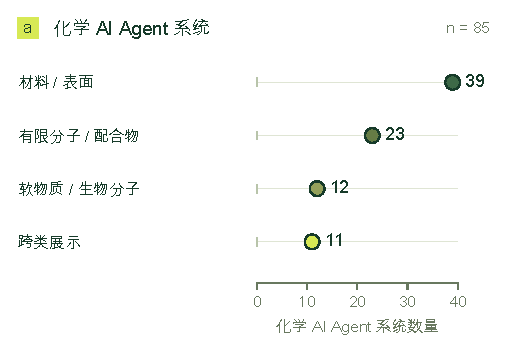
\includegraphics[width=\columnwidth]{figures/targets.pdf}
\caption{85个化学 AI Agent 系统的结构化文献样本：材料/表面39项、有限分子/配合物23项、软物质/生物分子12项、跨类系统11项。}
\label{fig:agent-targets}
\end{figure}


在几何推理层面，Cloudra 采用了“智能的克制”范式，将空间三维操作从大模型的认知负荷中剥离。系统将化学信息学结构感知与局部几何算子相衔接，最大公共子图（MCS）算法用于分子片段检索，原子映射和反应中心识别把分子拓扑连接与空间坐标紧密绑定；测量算子提供键长、键角、二面角与立体特征，局部操作算子则执行片段旋转、平移与过渡态装配。大语言模型无需猜测底层笛卡尔坐标，只需以清晰的化学意图发出结构变换指令，即可在可观测的几何变化中推进假设演化，削弱了人工对齐端点的必要性。

\begin{figure}[t]
\centering
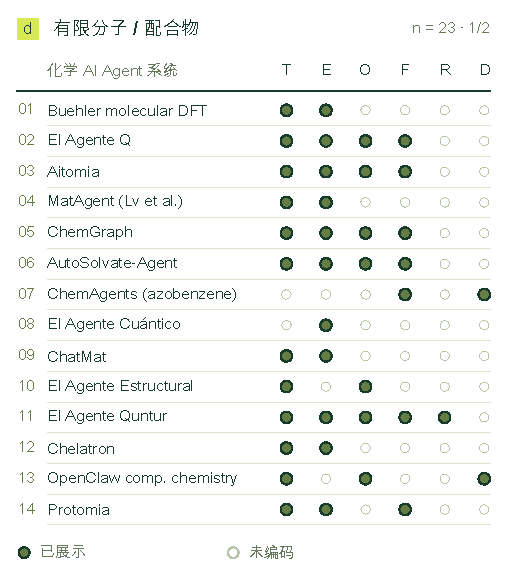
\includegraphics[width=\columnwidth]{figures/matrix_finite_molecules_complexes_01.pdf}
\caption{有限分子/配合物类已记录的任务（第1/2面板，共23个化学 AI Agent 系统）。T：结构构建/编辑；E：静态能量/性质；O：几何优化；F：振动/热化学；R：显式路径/过渡态；D：分子/量子动力学。实心表示正面证据，空白表示未编码，不代表缺少能力。}
\label{fig:agent-molecular-tasks-1}
\end{figure}


在科学交付层面，Cloudra 建立了以化学实体为核心的机理证据有向无环图（Delivery DAG）。与传统的任务调用流水线有着实质区别，Cloudra 交付图上的节点代表相应反应机理中的基态化学物种，边代表具有一阶鞍点（有且仅有一个有效虚频）和双向 IRC 路径完成验证的基元反应步骤。每一个科学主张的跃迁，都必须直接绑定底层真实的量子化学计算日志，而 Supervisor 门禁则依据科学的契约对交付图状态进行审核，确保程序性的判断错误没有被忽略。即使大模型在交互中宣称探索完成，若缺乏完整的频率或路径支撑，该步骤依然会被判定为未确证，抑制了虚假机理交付。

\begin{figure}[t]
\centering
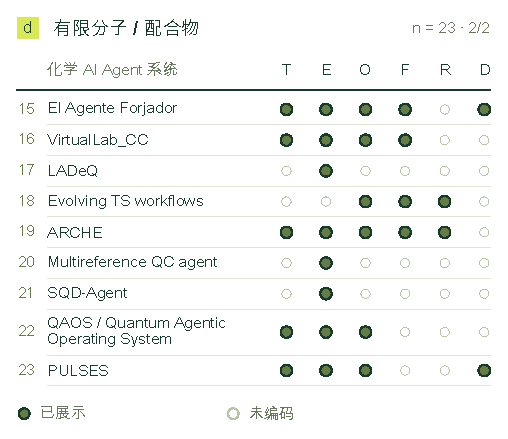
\includegraphics[width=\columnwidth]{figures/matrix_finite_molecules_complexes_02.pdf}
\caption{有限分子/配合物类化学 AI Agent 系统任务续图（第2/2面板），代码同图~\ref{fig:agent-molecular-tasks-1}。全部85个化学 AI Agent 系统的完整矩阵及逐项来源限制见配套材料。}
\label{fig:agent-molecular-tasks-2}
\end{figure}


\subsection{核心贡献}

Cloudra 提出了以化学物种与基元反应为实体、以物理化学法则为门禁的机理交付图（Delivery DAG）体系。通过将证据裁决权赋予底层的量化产物而非大模型的自然语言表述，系统从限制模型行为的角度抑制了语言模型在长程科学推理中的虚假完工与科学幻觉。

针对分子几何推理中普遍存在的人工干预与空间幻觉瓶颈，本文确立了“智能的克制”这一方法学范式。最大公共子图拓扑映射、立体位阻图遍历以及过渡态片段装配等几何操作被下沉为确定性算子，使大语言模型得以聚焦于高阶化学假说的提出、竞争通道抉择与失败归因，实现了复杂有机反应过渡态的端到端自主定位。

面向机理探索的严肃评测需求，本文构建了脱离主观打分、以原生计算产物为基准的反应机理评测体系（CloudraBench）。该基准涵盖 Easy、Normal、Hard 立体选择性竞争乃至 Impossible 物理不可达反应等五十道典型有机化学任务。通过跨两百个独立沙箱的四臂消融实验，评测直接从原生计算日志中提取，并由打分程序验证图结构覆盖度、物理自洽性以及定量能垒精度，为该领域确立了可复现的实证基线。

\bibliography{references}
\end{document}
